\documentclass[]{article}

\usepackage{indentfirst}
\usepackage{listings}
\usepackage{graphicx}
\usepackage{float}

\begin{document}
\title{Java 8 Parallel Streams}
\author{Ethan Williams}
\date{\today}
\maketitle

\tableofcontents

\section*{Prerequisites}
\subsection*{Technical}
This document was written for Java developers who have an interest in using concurrency (parallelism) in streams. Developers in other languages such as C\# may also find the topics useful with the understanding that syntax, implementation, and functionality may/will differ.

Additionally, the author assumes knowledge of serial streams in Java (the default stream implementation). Knowledge of concurrency tools/practices in Java is encouraged but not necessary.
\subsection*{Language}
Some of the language used in this paper may be ambiguous/confusing, the author's intended meanings for these terms are below:
\begin{itemize}
\item A stream instantiated with \verb|.stream()| only is referred to as a serial stream
\item A stream instantiated with \verb|.parallel().stream()| or \verb|.parallelStream()| is referred to as a parallel stream
\end{itemize}
\section{Introduction}
Parallel streams were introduced into Java 8 alongside serial streams so that developers could utilize concurrency to make stream processing faster. 
\section{Spliterator}
The Spliterator is the backbone of parallel streams, allowing the program to split a collection apart and iterate through it. If a collection object does not have a \verb|spliterator()| method returning a Spliterator object, then Java is not able to process the collection with a parallel stream at all.

\subsection{Basics}
A Spliterator is as an object which is represents the elements in a given range of the backing collection. At the beginning of a parallel stream there is one Spliterator that represents the entire collection. Calling the method \verb|trySplit()| will return a new Spliterator that represents the first half of untraversed elements while modifying the instance to represent the second half of untraversed elements. Figure \ref{fig:split} illustrates a call to \verb|trySplit()| on a Spliterator representing the entire collection.

\begin{figure}[H]
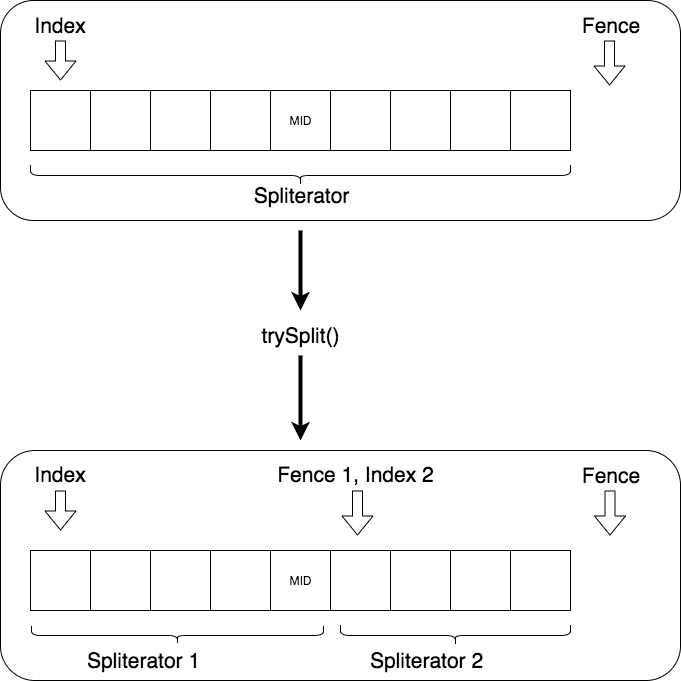
\includegraphics[width=\linewidth]{images/spliterator_illustrated.png}
\caption{A Spliterator before and after splitting}
\label{fig:split}
\end{figure}

\subsection{Implementation}
\textit{Spliterator implementations differ based on the collection so this section focuses on a simplified (easier to read) implementation of the Spliterator for Java's ArrayList.}

 Spliterator has 3 instance fields: a backing collection, an index, and a fence. The backing collection for every Spliterator the entire collection it is based on. The index is the current cursor position of the Spliterator, which is analogous to the cursor position in an Iterator object. The fence is the index of the last element the Spliterator is responsible for plus one. The primary methods are \verb|tryEachRemaining()|, \verb|tryNext()|, \& \verb|trySplit()|. 

Although the cursor is similar to Iterator's, traversal through a Spliterator using \verb|tryEachRemaining()| and \verb|tryNext()| is different. \verb|tryEachRemaining()| in Figure \ref{fig:forEachRemaining} takes a Consumer object which is the operation to be carried out on each element of the collection. A typical implementation will simply iterate through all elements and call the \verb|accept()| method on the consumer with the element as its only parameter. \verb|tryNext()| in Figure \ref{fig:tryAdvance} is similar although the operation is only attempted on element at the current cursor position. If that cursor position is past the fence of the Spliterator, then the method returns false, otherwise it returns true.

\begin{figure}[H]
\begin{lstlisting}[language=Java]
public void forEachRemaining(Consumer<? super E> action) {
    int i;
    if ((i = index) >= 0 && (index = fence) <= a.length) {
        for (; i < hi; ++i)  action.accept((E) list.elementData[i]);
    }
    throw new ConcurrentModificationException();
}
\end{lstlisting}
\caption{Implementation of forEachRemaining()}
\label{fig:forEachRemaining}
\end{figure}

\begin{figure}[H]
\begin{lstlisting}[language=Java]
public boolean tryAdvance(Consumer<? super E> action) {
    int hi = getFence(), i = index;
    if (i < hi) {
        index = i + 1;
        action.accept((E) list.elementData[i]);
        return true;
    }
    return false;
}
\end{lstlisting}
\caption{Implementation of tryAdvance()}
\label{fig:tryAdvance}
\end{figure}

Spliterator's primary functionality is encapsulated within the \verb|trySplit()| method in Figure \ref{fig:trySplit}

\begin{figure}[H]
\begin{lstlisting}[language=Java]
public Spliterator<E> trySplit() {
    int lo = index, mid = (lo + fence) >>> 1;
    return (lo >= mid) ? null : new Spliterator<E>(list, lo, index = mid);
}
\end{lstlisting}
\caption{Implementation of trySplit()}
\label{fig:trySplit}
\end{figure}
\section{Collectors}
\section{Practical Considerations when Using Parallel Streams}
\end{document}

\end{document}